\begin{flushleft}
\doublespacing

\subsection{JUnit tests}
\subsection{Brugertest}

\begin{figure}[htp] %brug begin{figure} til alle figurer.
    \centering
    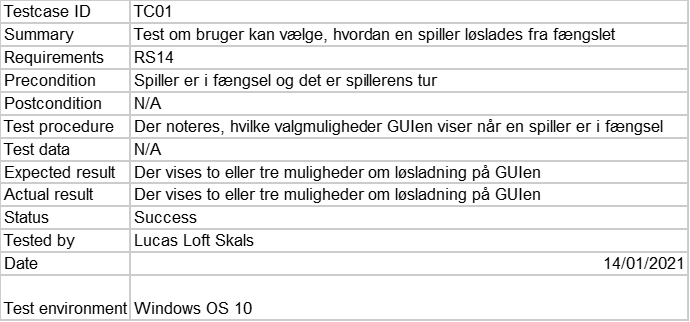
\includegraphics[width=14cm]{Report/figures/Usertests/TC01.png}
    \caption{Tabel over TC01}
    \label{Testcase01}
\end{figure}

\begin{figure}[htp] %brug begin{figure} til alle figurer.
    \centering
    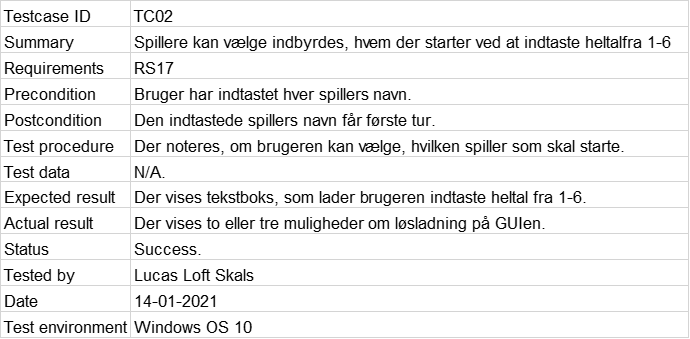
\includegraphics[width=14cm]{Report/figures/Usertests/TC02.png}
    \caption{Tabel over TC02}
    \label{Testcase02}
\end{figure}

\begin{figure}[htp] %brug begin{figure} til alle figurer.
    \centering
    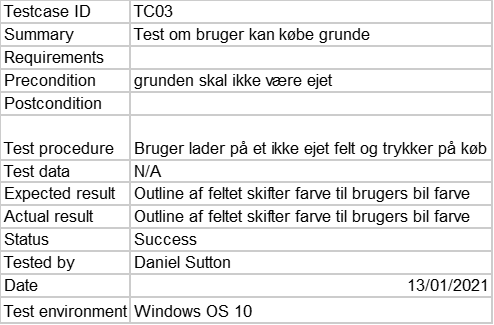
\includegraphics[width=14cm]{Report/figures/Usertests/TC03.png}
    \caption{Tabel over TC03}
    \label{Testcase03}
\end{figure}

\end{flushleft}